% !TEX root = SFV-14033_SFT1.tex
\section{Pr\"aliminarien}

%\begin{frame}[plain]
%\begin{center}
%\vspace{2cm}
%\Huge Warum seid Ihr heute hier?\\ \vspace{.5cm}
%\pause \Large Die Zahlentheorie ist nützlich, weil man mit ihr promovieren kann.\\
%Edmund Landau
%\end{center}
%\end{frame}


\begin{frame} % Cover slide
\titlepage
\end{frame}

\frame{\sectionpage}

\frame{\frametitle{Prof. Dr. Raphael Pfaff}
\framesubtitle{Lehr- und Forschungsgebiet Schienenfahrzeugtechnik}
\begin{columns}[t] 
     \begin{column}[T]{7cm} 
     	\begin{itemize}
		\item[] \includegraphics[width=0.4cm]{Email} \hspace{.1cm} pfaff@fh-aachen.de
		\item[] \includegraphics[width=0.4cm]{Twitter} \hspace{.1cm} @RailProfAC
		\item[] \includegraphics[width=0.4cm]{Wordpress} \hspace{.1cm} www.raphaelpfaff.net
		\item[] Prezume: \texttt{\url{http://goo.gl/iq6lhh}}
		\vspace{1cm}
		\item Raum 02305
		\item Sprechstunde nach Vereinbarung
     	\end{itemize}
	
     \end{column}
     	\begin{column}[T]{5cm} 
         	\begin{center}
            		\includegraphics[width=0.8\textwidth]{Profilklein}
        		\end{center}
     \end{column}
 \end{columns}
}

\frame{\frametitle{Vorstellungsrunde}
\framesubtitle{}
\begin{itemize}
\item Wer bist Du?
\item Was erwartest Du von SFT1?
\item Was kann ich tun, damit SFT1 Dein Traummodul wird?
\item Was muss ich tun, damit Du SFT1 hasst?
\end{itemize}
}


\frame{\frametitle{Anforderungen ``First Cycle'' - Bachelor}
\framesubtitle{Anforderungen gem\"a{\ss} Dublin Descriptors}
\begin{columns}[t] 
     \begin{column}[T]{7cm} 
     	\begin{itemize}
     		\item Knowledge and understanding in a field of study
		\begin{itemize}
		\item Typically supported by textbooks
		\item Some aspects informed by knowledge on the forefront of the field of study
		\end{itemize}
		\item Apply knowledge and understanding indicating a professional approach
		\item Gather and interpret data to inform judgement
		\item Communicate information, ideas, problems and solutions
		\item Learning skills to undertake further study with high degree of autonomy
     	\end{itemize}
     \end{column}
     	\begin{column}[T]{5cm} 
         	\begin{center}
	\vspace{1cm}
            		\includegraphics[width=0.8\textwidth]{GraduationHat}
        		\end{center}
     \end{column}
 \end{columns}
}

\frame{\frametitle{Anforderungen ``Niveau 6'' - Bachelor}
\framesubtitle{Anforderungen gem\"a{\ss} Deutschem Qualifizierungsrahmen}
\begin{columns}[t] 
     \begin{column}[T]{7cm} 
     	\begin{itemize}
     		\item Breites und integriertes Wissen
		\begin{itemize}
		\item Wissenschaftliche Grundlagen
		\item Praktische Anwendungen 
		\end{itemize}
		\item Breites Spektrum an Methoden
		\begin{itemize}
		\item Neue L\"osungen erarbeiten und bewerten
		\end{itemize}
		\item Verantwortlich in Expertenteams arbeiten oder leiten
		\item Ziele f\"ur Lern- und Arbeitsprozesse definieren, reflektieren und bewerten
		\item Lern- und Arbeitsprozesse eigenst\"andig und nachhaltig gestalten
     	\end{itemize}
     \end{column}
     	\begin{column}[T]{5cm} 
         	\begin{center}
	\vspace{1cm}
            		\includegraphics[width=0.8\textwidth]{GraduationHat}
        		\end{center}
     \end{column}
 \end{columns}
}


\frame{\frametitle{Anforderungen BEng Schienenfahrzeugtechnik}
\framesubtitle{Was zeichnet einen Bachelor der Schienenfahrzeugtechnik aus?}
\begin{columns}[t] 
     \begin{column}[T]{6cm} 
     	\begin{itemize}
		\item Wissenschaftliches Arbeiten
		\begin{itemize}
		\item Nutzung Prim\"arliteratur und Normen
		\item Erstellung Seminararbeiten
		\end{itemize}
     		\item Selbstlernkompetenz
		\begin{itemize}
		\item Beispiel: Nutzung Lehrbuch statt Skript
		\end{itemize}
		\item Verfassung wissenschaftlicher und technischer Texte
		\item Fachvortrag zu Seminararbeit
     	\end{itemize}
     \end{column}
     	\begin{column}[T]{6cm} 
         	\begin{center}
	\vspace{1cm}
            		\includegraphics[width=0.8\textwidth]{GraduationHat}
        		\end{center}
     \end{column}
 \end{columns}
}

\frame{\frametitle{Wie schaffen? - Growth Mindset!}
\framesubtitle{Theorie der Psychologin Carol Dweck, Harvard \cite{mindset}}
\begin{columns}[t] 
     \begin{column}[T]{6cm} 
     \textbf{Fixed Mindset:} 
     	\begin{itemize}
     		\item F\"ahigkeiten,
		\item Intelligenz und
		\item Talent 
     	\end{itemize}
	sind feste Pers\"onlichkeitsmerkmale und nicht \"anderbar. Daher das Bestreben, nicht dumm zu wirken.
     \end{column}
     	\begin{column}[T]{6cm} 
	\textbf{Growth Mindset:} 
         	\begin{itemize}
     		\item F\"ahigkeiten,
		\item Intelligenz und
		\item Talent 
     		\end{itemize}
		k\"onnen durch Anstrengung, gute Lehre und Hartn\"ackigkeit entwickelt werden. Nicht jeder ist gleich, aber jeder kann sich weiterentwickeln.
     \end{column}
 \end{columns}
}

\frame{\frametitle{Entwicklung im Growth Mindset}
\framesubtitle{}
\begin{center}
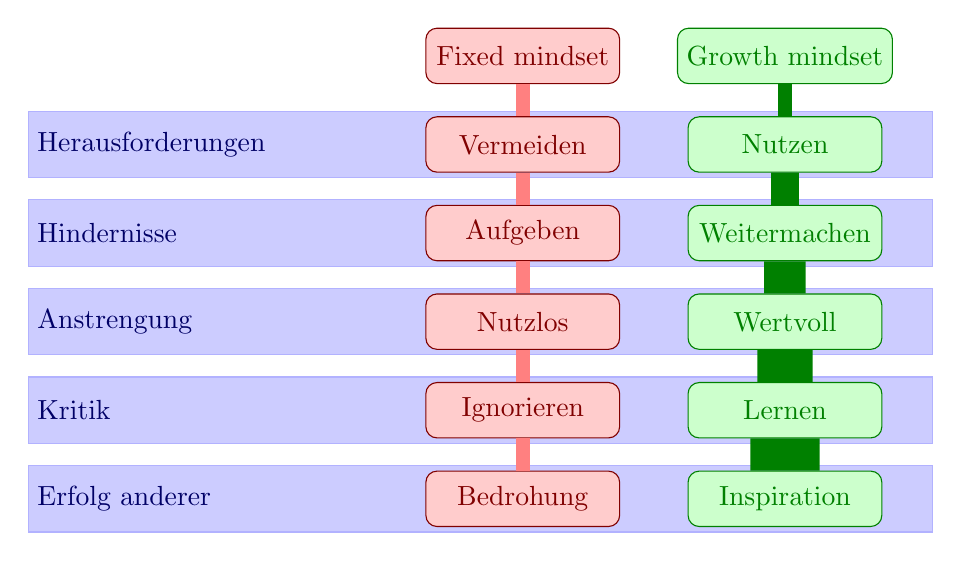
\begin{tikzpicture}[scale = .9, minimum height = 20]
\node (fixed)[minimum width = 70, draw=red!50!black, fill = red!20, rounded corners] at ( .6,8.75) {\textcolor{red!50!black}{Fixed mindset}};
\node (growth)[minimum width = 70, draw=green!50!black, fill = green!20, rounded corners]  at ( 4.3,8.75){\textcolor{green!50!black}{Growth mindset}};

\node (challenges)[text width = 320, draw=blue!30, fill = blue!20, align = left, minimum height = 24] at ( 0,7.5) {\textcolor{blue!40!black}{Herausforderungen}};
\node (obstacles)[text width = 320, draw=blue!30, fill = blue!20, align = left, minimum height = 24] at ( 0,6.25) {\textcolor{blue!40!black}{Hindernisse}};
\node (effort)[text width = 320, draw=blue!30, fill = blue!20, align = left, minimum height = 24] at ( 0,5) {\textcolor{blue!40!black}{Anstrengung}};
\node (criticism)[text width = 320, draw=blue!30, fill = blue!20, align = left, minimum height = 24] at ( 0,3.75) {\textcolor{blue!40!black}{Kritik}};
\node (success)[text width = 320, draw=blue!30, fill = blue!20, align = left, minimum height = 24] at ( 0,2.5) {\textcolor{blue!40!black}{Erfolg anderer}};

\begin{scope}[draw = red!50!black]
\uncover<2-7>{\node (avoid)[minimum width = 70, draw, fill = red!20, rounded corners] at ( .6,7.5) {\textcolor{red!50!black}{Vermeiden}};
\path[draw, draw=red!50, line width = 5pt] (fixed) -- (avoid);};
\uncover<3-7>{\node (giveup)[minimum width = 70, draw, fill = red!20, rounded corners] at ( .6,6.25) {\textcolor{red!50!black}{Aufgeben}};
\path[draw, draw=red!50, line width = 5pt] (avoid) -- (giveup);};
\uncover<4-7>{\node (useless)[minimum width = 70, draw, fill = red!20, rounded corners] at ( .6,5) {\textcolor{red!50!black}{Nutzlos}};
\path[draw, draw=red!50, line width = 5pt] (giveup) -- (useless);};
\uncover<5-7>{\node (ignore)[minimum width = 70, draw, fill = red!20, rounded corners] at ( .6,3.75) {\textcolor{red!50!black}{Ignorieren}};
\path[draw, draw=red!50, line width = 5pt] (useless) -- (ignore);};
\uncover<6-7>{\node (threat)[minimum width = 70, draw, fill = red!20, rounded corners] at ( .6,2.5) {\textcolor{red!50!black}{Bedrohung}};
\path[draw, draw=red!50, line width = 5pt] (ignore) -- (threat);};
\end{scope}

\begin{scope}[draw = green!50!black]
\uncover<2-7>{\node (embrace)[draw, minimum width = 70, fill = green!20, rounded corners] at ( 4.3,7.5) {\textcolor{green!50!black}{Nutzen}};
\path[draw,  line width = 5pt] (growth) -- (embrace);};
\uncover<3-7>{\node (persist)[draw, minimum width = 70,  fill = green!20, rounded corners] at (4.3,6.25) {\textcolor{green!50!black}{Weitermachen}};
\path[draw,  line width = 10pt] (embrace) -- (persist);};
\uncover<4-7>{\node (valuable)[draw, minimum width = 70,  fill = green!20, rounded corners] at ( 4.3,5) {\textcolor{green!50!black}{Wertvoll}};
\path[draw,  line width = 15pt] (persist) -- (valuable);};
\uncover<5-7>{\node (learn)[draw, minimum width = 70,  fill = green!20, rounded corners] at ( 4.3,3.75) {\textcolor{green!50!black}{Lernen}};
\path[draw,  line width = 20pt] (valuable) -- (learn);};
\uncover<6-7>{\node (inspiration)[draw, minimum width = 70,  fill = green!20, rounded corners] at (4.3,2.5) {\textcolor{green!50!black}{Inspiration}};
\path[draw,  line width = 25pt] (learn) -- (inspiration);};
\end{scope}

\end{tikzpicture}
\end{center}
}

\frame{\frametitle{Rolle des Lehrenden}
\framesubtitle{}
\begin{columns}[t] 
     \begin{column}[T]{6cm} 
     \vspace{1cm}
     	\begin{quote}
     		A teacher is never a giver of truth; he is a guide, a pointer to the truth that each student must find for himself.
     	\end{quote}
	\flushright Bruce Lee
	
     \end{column}
     	\begin{column}[T]{6cm} 
         	\begin{center}
            		\includegraphics[width=0.8\textwidth]{Bruce}
        		\end{center}
     \end{column}
 \end{columns}
}


\frame[allowframebreaks]{
\frametitle{Inhalt der Vorlesung}
\tableofcontents
}


\frame{\frametitle{Vorlesungsinhalte}
\framesubtitle{}
\begin{center}
\begin{tikzpicture}[scale = 0.95, small mindmap, concept color=gray!30]
\node [concept] {Schienen-fahrzeug-technik}
child [grow = 0]{node[concept] {Grundlagen}
child [grow = -30] {node[concept] {Systematik}}
child [grow = 30]{node[concept] {Normen und Regeln}}}
child [grow = 60]{node[concept] {Anfor-derungen}
child [grow = -20] {node[concept] {Requirements Engineering}}
child [grow = 20]{node[concept] {Lebenszyklus}}}
child [grow = 130]{node[concept] {Fahrzeuge}
child [grow = 30] {node[concept] {G\"uterwagen}}
child [grow = 150]{node[concept] {Personen-fahrzeuge}}
child [grow = 190]{node[concept] {Triebfahr-zeuge}}}
child [grow = 180]{node[concept] {Zugf\"order-technik}
child [grow = 160] {node[concept] {Spurf\"uhrung}}
child [grow = 200]{node[concept] {Rad-Schiene-Kontakt}}}
child [grow = 235]{node[concept] {Fahrzeug-konstruk-tion}
child [grow = 160] {node[concept] {Bauformen}}
child [grow = 200]{node[concept] {Mechanischer Aufbau}}}
child [grow = 300]{node[concept] {Laufwerk}
child [grow = 20] {node[concept] {Drehgestell}}
child [grow = 210]{node[concept] {Radsatz}}
child [grow = -20]{node[concept] {Federn und D\"ampfer}}
};
\end{tikzpicture}
\end{center}
}

\offslide{Fehlt etwas?}{Was k\"onnt Ihr noch gebrauchen? z.B. f\"ur die Railway Challenge, euer Mobilit\"atsfenster, ...}


\frame{\frametitle{Themenplan}
\framesubtitle{Das Lehrbuch von \emph{Janicki} et al. \citep{janicki} ist Pflichtlekt\"ure in diesem Modul, f\"ur weitere vertiefende Literatur siehe Literaturverzeichnis. Vorschl\"age f\"ur Themen der Seminararbeit sind willkommen!}
%\tiny
\hspace{1cm}
\begin{tabular}{|l|l|}
\hline
Thema & Kapitel aus \citep{janicki}\\ 
Pr\"aliminarien,  G\"uterwagen, Personenfahrzeuge& 6, 7.1\\ \hline
Einf\"uhrung Zugdynamik & 1.5.1, 1.5.2, 2.4 \\ \hline
Zugdynamik - Einf\"uhrung, Kraftschluss, Schlupf &  1.5.2 \\ 
Zugdynamik II - Fahrwiderstand, Zugkraft, Zugbremsung & 1.5, 5.2   \\ \hline
Einf\"uhrung Spurf\"uhrung & 1.4   \\ \hline
Kuppelsto{\ss}, Crash &   \\ \hline
Fahrzeugkonstruktion & 2.1.1 - 2.1.9  \\
Bauformen, Begrenzungen, Aufbau &  \\ 
Werkstoffe, F\"ugetechnik, &     \\
Brandschutz, Passive Safety &   \\ \hline
Laufwerke  & 2.2.1 - 2.2.13   \\
Einf\"uhrung, Radsatz, Drehgestell &  \\ 
Federung, D\"ampfung, Anbauten &  \\ \hline 
\end{tabular}
}

\frame{\frametitle{Semesterbegleitende Pr\"ufung, Praktikum}
\framesubtitle{}
\only<1>{
\begin{itemize}
\item Anhand Railway Challenge und \textit{Service Learning} f\"ur EVS
\begin{itemize}
	\item Aufgaben werden abgestimmt
\end{itemize}
\item Dokumentation durch technische Berichte
\item Gewichtung Berichte: in Summe 100\% der Modulnote
\end{itemize}}
\only<2>{
\begin{center}
\includegraphics[width = 7.5cm]{SFT1Plan}
\end{center}
}
}



